\chapter{验证方法与工作概述}
\section{形式化验证实施流程}
\label{sec:verification-process}

\subsection{核心验证流程}
\label{subsec:core-flow}

本研究验证流程如下图所示,包含以下三个关键阶段:
\begin{figure}[h]
    \centering
    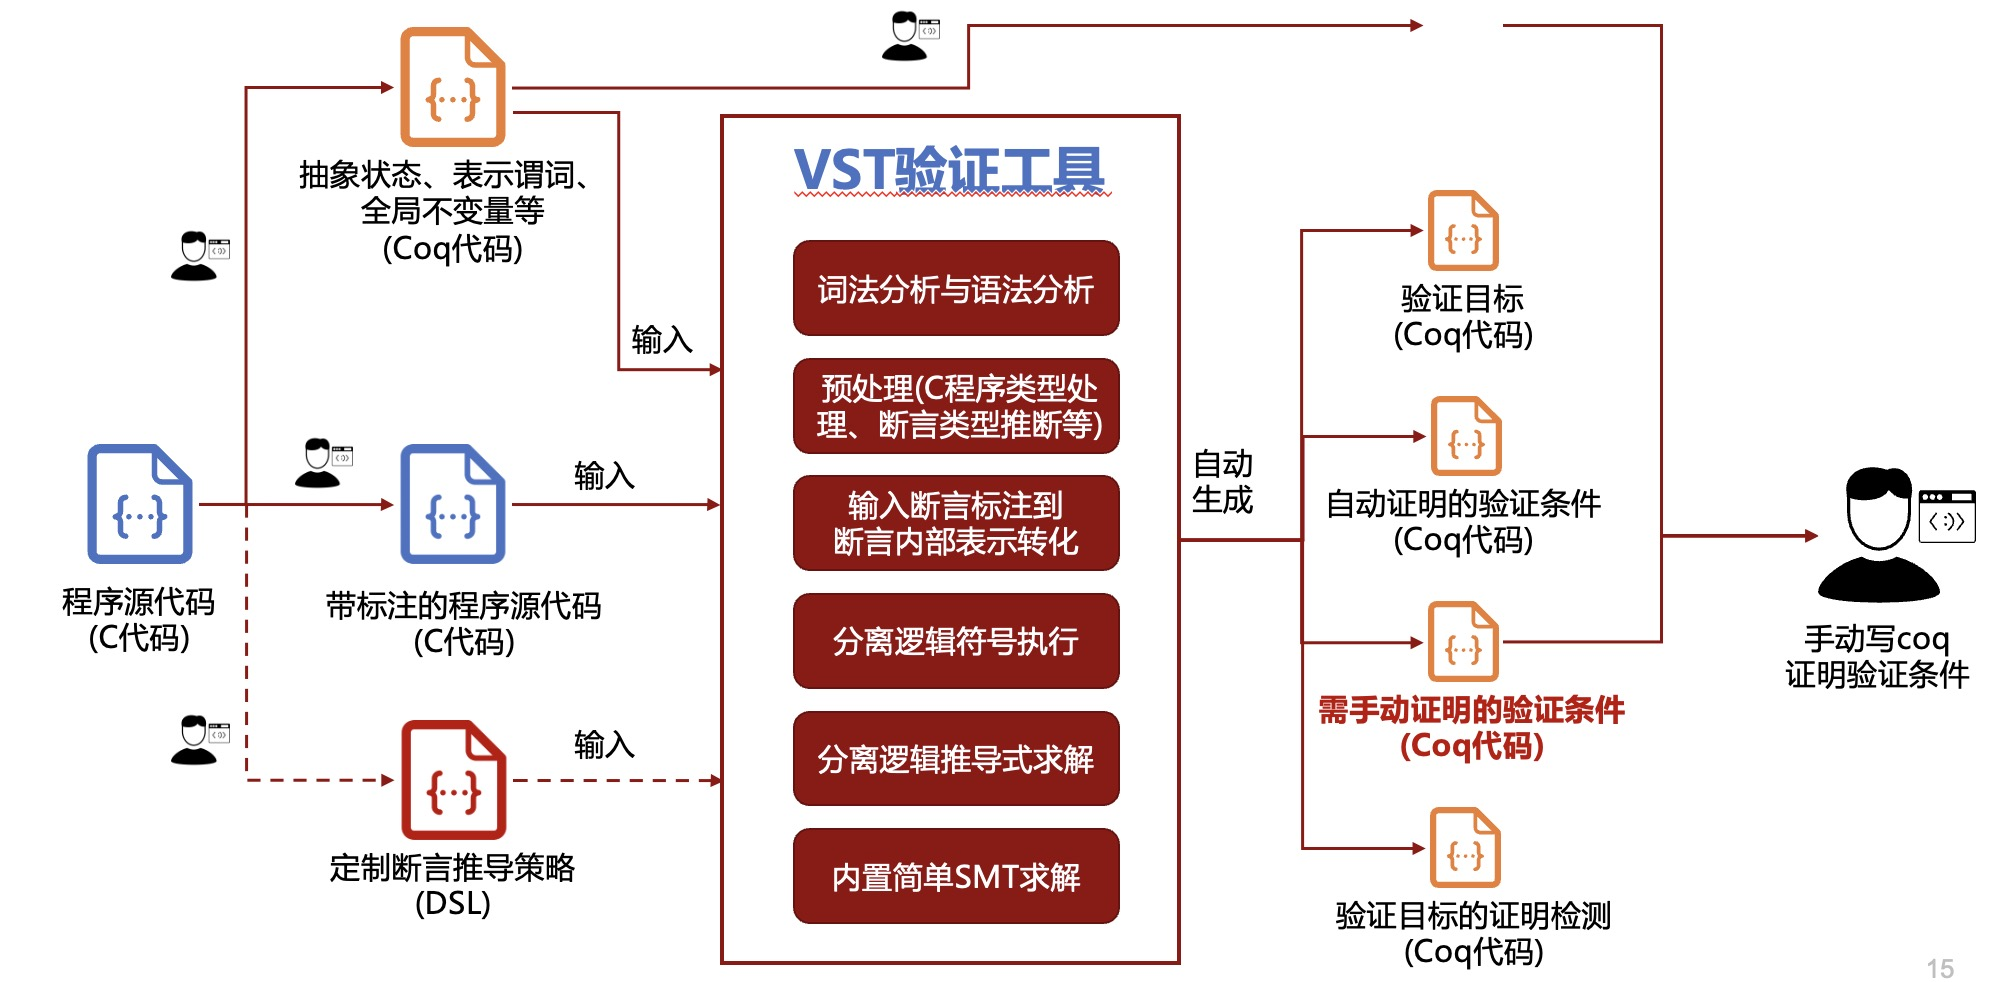
\includegraphics[width=0.9\textwidth]{./fig/vst-flow.png}
    \caption{验证流程核心阶段示意图}
    \label{fig:vst-flow}
\end{figure}

\begin{itemize}
    \item \textbf{建模规约}
    \begin{itemize}
        \item 在Coq中定义数据结构的内存模型(如链表、缓冲区等);
        \item 建立全局不变量与函数级形式化规约;
        \item 编制strategy,指导VST执行验证策略,简化验证过程;
    \end{itemize}

    \item \textbf{自动化验证}
    \begin{itemize}
        \item 通过VST执行符号生成验证条件;
        \item 应用内置SMT求解器处理基础约束;
    \end{itemize}

    \item \textbf{人工介入}
    \begin{itemize}
        \item 处理VST执行符号执行后无法自动证明的验证;
        \item 编写Coq证明脚本,完成复杂验证条件的证明;
    \end{itemize}
\end{itemize}

\subsection{分离逻辑与VST应用}
\label{subsec:sep-vst}

本研究采用VST验证工具实施程序验证,具体流程包含以下三个阶段,各阶段需研究者完成的核心任务如下:

\subsection{建模规约阶段}
\label{subsec:preparation}
本阶段在Coq中建立程序的形式化模型,具体实施包含以下核心内容:
\begin{enumerate}
    \item \textbf{数据结构建模}
    \begin{itemize}
        \item 在Coq中定义C数据结构:
        \begin{figure}[h]  % 位置参数:h此处,t顶部,b底部,p独立页
            \centering  % 居中图片
            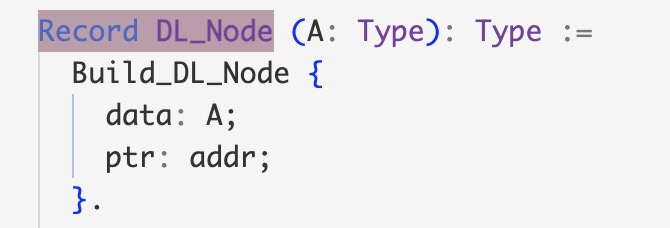
\includegraphics[width=0.8\textwidth]{./fig/Record_dll.png}  % 调整宽度为文本宽度的80%
            \caption{双向链表定义}  % 图片标题
            \label{fig:Record_dll}  % 用于交叉引用的标签
        \end{figure}
        \item 在Coq中定义全局不变量:
        \begin{figure}[h]  % 位置参数:h此处,t顶部,b底部,p独立页
            \centering  % 居中图片
            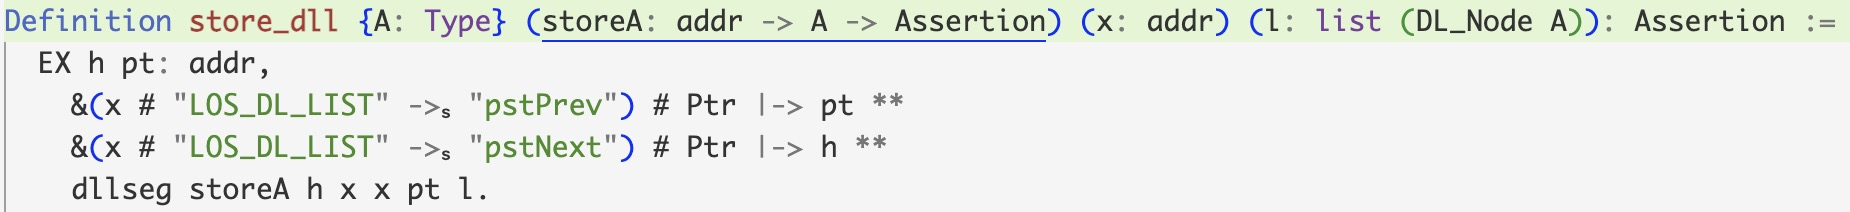
\includegraphics[width=0.8\textwidth]{./fig/store_dll.png}  % 调整宽度为文本宽度的80%
            \caption{store\_dl函数定义与断言示意图}  % 图片标题
            \label{fig:store-dl}  % 用于交叉引用的标签
        \end{figure}
        \item 在C源代码中插入形式化标注:
        \begin{figure}[h]  % 位置参数:h此处,t顶部,b底部,p独立页
            \centering  % 居中图片
            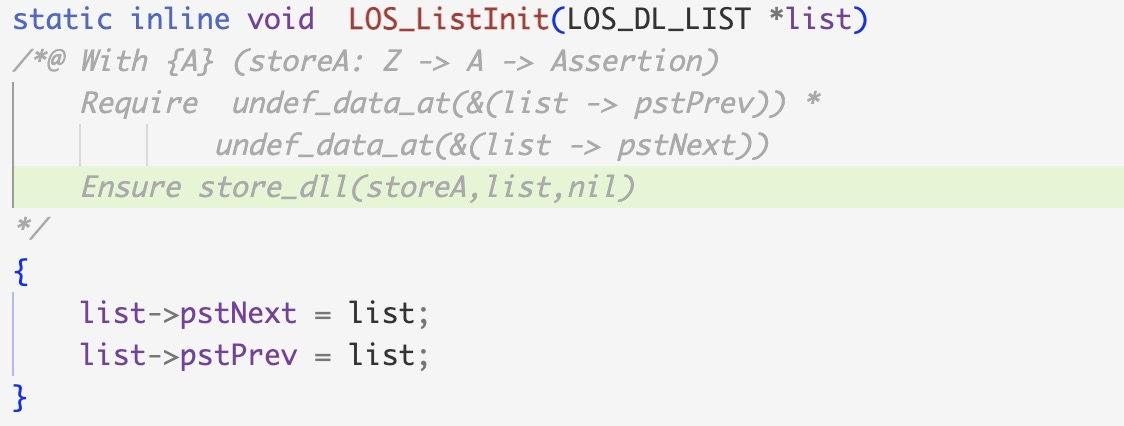
\includegraphics[width=0.8\textwidth]{./fig/LOS_ListInit.png}  % 调整宽度为文本宽度的80%
            \caption{函数形式化标注}  % 图片标题
            \label{fig:LOS_ListInit}  % 用于交叉引用的标签
        \end{figure}
        \item 编写VST验证推导策略:
        \begin{figure}[H]  % 位置参数:h此处,t顶部,b底部,p独立页
            \centering  % 居中图片
            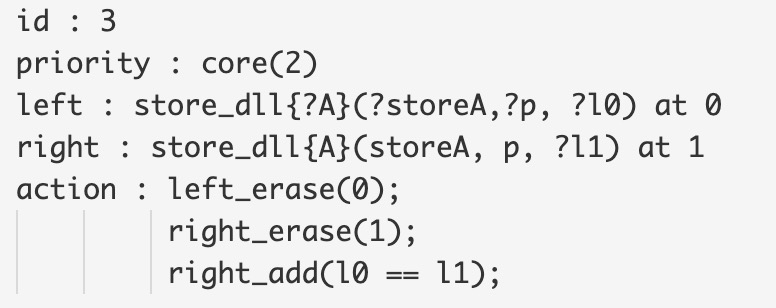
\includegraphics[width=0.8\textwidth]{./fig/store_dll_strategy.png}  % 调整宽度为文本宽度的80%
            \caption{VST Strategy}  % 图片标题
            \label{fig:store_dll_strategy}  % 用于交叉引用的标签
        \end{figure}
    \end{itemize}
\end{enumerate}

\subsection{验证执行阶段}
\label{subsec:execution}

本阶段通过VST工具实现程序验证,具体流程如下:

\begin{enumerate}
    \item \textbf{验证文件生成}
    \begin{itemize}
        \item 输入标注的C代码与验证策略后,生成四类核心文件:
        \begin{itemize}
            \item \texttt{xxx\_proof\_goal}:所有待证明结论列表
            \item \texttt{xxx\_proof\_auto}:已经通过strategy和SMT solver自动解决的相关证明
            \item \texttt{xxx\_proof\_manual}:需要手动完成的相关证明
            \item \texttt{xxx\_proof\_check}:所有证明都已经完成的检查文件汇总
        \end{itemize}
    \end{itemize}

    \item \textbf{自动验证处理}
    \begin{itemize}
        \item 内置符号执行引擎遍历程序路径
        \item 应用验证策略处理基础验证(如内存地址有效性验证)
    \end{itemize}

    \item \textbf{人工验证实施}
    \begin{itemize}
        \item 使用Coq对较复杂的SMT无法自动完成验证的条件进行验证。
        \item 将多个函数的证明合并在一起之后使用Coq进行统一验证,以确保整个系统各个函数调用时系统的正确性。
    \end{itemize}
\end{enumerate}

\section{操作系统建模与形式化规约}
\subsection{内存管理模块的形式化验证}

\noindent VST-IDE通过分离逻辑对动态内存管理进行形式化规约与验证,具体流程如下:

\subsubsection{堆分配器规约}
\begin{equation}
\hoare{\mathrm{emp}}{\mathtt{malloc}(n)}{\exists p.\ \mathrm{valid\_ptr}(p) \ast \mathrm{block}(p, n)}
\end{equation}
\noindent 其中:
\begin{itemize}
    \item $\mathrm{emp}$ 表示空堆断言
    \item $\mathrm{valid\_ptr}(p)$ 保证指针$p$的有效性
    \item $\mathrm{block}(p, n)$ 声明$p$指向大小为$n$字节的连续内存块
    \item $\ast$ 为分离逻辑合取运算符
\end{itemize}

\subsubsection{自动化验证实现}
生成Coq验证代码:
\begin{itemize}
    \item \texttt{*\_proof\_goal.v}(VST-IDE生成的验证目标)
    \item \texttt{*\_proof\_auto.v}(VST-IDE自动证明的命题)
    \item \texttt{*\_proof\_manual.v}(用户使用Coq交互式证明器需要证明的命题)
\end{itemize}

\subsection{进程隔离机制的验证方法}
\label{subsec:proc-isolation}

\subsubsection{能力模型(Capability Model)}
\label{subsubsec:capability-model}

\noindent 定义进程资源归属谓词:
\begin{equation}
\mathrm{ProcRes}(p) \triangleq \ast_{r \in \mathrm{Res}(p)} \mathrm{own}(r,\,p)
\end{equation}
\noindent 其中:
\begin{itemize}
    \item $\mathrm{Res}(p)$ 表示进程$p$拥有的资源集合
    \item $\mathrm{own}(r,\,p)$ 声明资源$r$归属进程$p$,满足:
        \begin{equation}
        \mathrm{own}(r,\,p) \triangleq r \hookrightarrow_p \mathrm{meta}(p)
        \end{equation}
    \item $\ast$ 为分离逻辑的迭代合取运算符,满足:
        \begin{equation}
        \ast_{i=1}^n P_i \equiv P_1 \ast \cdots \ast P_n
        \end{equation}
\end{itemize}

\subsubsection{隔离性定理}
\begin{equation}
\forall p_1 \neq p_2,\ \mathrm{ProcRes}(p_1) \ast \mathrm{ProcRes}(p_2) \vdash \bot
\end{equation}
\noindent 该定理保证:
\begin{itemize}
    \item 分离性:$\mathrm{Res}(p_1) \cap \mathrm{Res}(p_2) = \emptyset$,进程间资源互斥
    \item 无干扰性:进程无法访问不归属于自己的资源
\end{itemize}
\subsection{循环不变式描述}
\section*{程序状态形式化描述}

首先,循环不变式有两条必须满足的性质,即可达性和归纳性。此外,在程序验证中,我们一般还要求循环不变式可证明需要验证的属性。接下来,我们将使用以下的例子,结合形式化的定义,来介绍以上这些性质。

\begin{lstlisting}[language=C++, caption=示例程序]
// to ten
int i = 0;
while(i < 10) { // Inv(i): 0 <= i <= 10
    i = i + 1;
}
assert(i == 10);
\end{lstlisting}

为了形式化地定义循环不变式,我们先做以下定义:

\begin{itemize}
    \item 用 $X$ 来表示程序变量的值,$X$ 可以被理解成一个由程序中所有变量组成的元组(Tuple),或者向量(Vector)
    
    \item 用 $Pre(X)$ 表示循环前的代码对程序变量值的约束
    
    \item 用 $Inv(X)$ 表示循环不变式对程序变量值的约束
    
    \item 用 $G(X)$(Guard)表示循环条件对程序变量值的约束
    
    \item 用 $T(X, X')$ 表示循环体代码对程序变量值的修改,其中 $X'$ 表示被循环体修改后的程序变量的值
    
    \item 用 $Post(X)$ 表示循环后的代码对程序变量值的约束,一般为所需要验证的属性对程序变量值的要求
\end{itemize}
\subsection*{可达性}
可达性实质上是要求,循环不变式表示的状态集合,即$\mathit{Inv}(X)$应该包含所有经过循环前的代码所能到达的状态所形成的集合,即状态集合$\mathit{Pre}(X)$。

\begin{equation}
\forall X.\; \mathit{Pre}(X) \Rightarrow \mathit{Inv}(X)
\end{equation}

\paragraph{示例}
在这个例子中,循环头前的代码形成的约束为$i = 0$。这就意味着,不变式应该包含所有满足$i = 0$的状态。事实上,$0 \leq i \leq 10$包含$i = 0$,即:
$$
\{0\} \subset \{0, 1, \ldots, 10\}
$$
因此可达性成立。

\begin{equation}
\forall i.\; (i = 0) \Rightarrow (0 \leq i \leq 10)
\end{equation}

\subsection*{归纳性}
归纳性是循环不变式最重要的性质,它要求任何被包含在循环不变式中的状态,经过循环后,得到的新状态仍然落在循环不变式中。这个性质保证了循环不变式在任意次循环执行后始终成立。

\begin{equation}
\forall X,X'.\; \left( \mathit{Inv}(X) \land G(X) \land T(X,X') \right) \Rightarrow \mathit{Inv}(X')
\end{equation}

\paragraph{示例验证}
在示例程序中,循环不变式 $0 \leq i \leq 10$ 对应的状态集合为 $\{0,1,\ldots,10\}$。取其中满足循环条件 $i<10$ 的状态 $i=1$,经过循环体后得到 $i'=2$,仍然满足:

$$
\{2\} \subseteq \{0,1,\ldots,10\}
$$

使用逻辑公式验证该不变式的归纳性:
\begin{align*}
\forall i.\; &(0 \leq i \leq 10 \land i < 10) \\
&\Rightarrow 0 \leq i+1 \leq 10
\end{align*}

\paragraph{重要结论}
满足归纳性的不变式可能有多个,但需选择能验证程序属性的:
\begin{itemize}
    \item \textbf{有效不变式}:$0 \leq i \leq 10$ 和 $i \leq 10$ 均可证明 \texttt{assert(i==10)}
    \item \textbf{无效不变式}:$i \leq 20$ 满足可达性和归纳性,但无法证明最终状态 $i=10$
\end{itemize}

\subsection*{可证明性}
该性质要求当循环不变式中的状态满足循环终止条件时,必须满足待验证的程序属性。形式化定义为:

\begin{equation}
\forall X.\; \mathit{Inv}(X) \land \neg G(X) \Rightarrow \mathit{Post}(X)
\end{equation}

\paragraph{示例验证}
在示例程序中,应用具体参数得到验证式:
\begin{align*}
\forall i.\; &(0 \leq i \leq 10) \land \neg(i < 10) \\
&\Rightarrow (i = 10)
\end{align*}

\paragraph{逻辑等价转换} 该式可简化为:
$$
\forall i.\; (0 \leq i \leq 10) \land (i \geq 10) \Rightarrow (i = 10)
$$
在整数域上,该蕴含式等价于:
$$
\{10\} \subseteq \{10\}
$$
因此公式有效。

\subsection{操作规约}
\section{基于VST验证流程}
\subsection{操作系统资源建模}
\subsection{函数条件与断言}
\subsection{验证过程与结果分析}
\section{主要验证内容}
\subsection{基本数据结构-链表}
\subsection{基于链表的操作系统核心模块}
\section{本章小结}
% vim:ts=4:sw=4